\section{Experiments \label{sec:expts}}   
We perform experiments with five  GP models: standard regression \cite{rasmussen-williams-book}, warped GPs \cite{snelson2003warped}, binary classification \cite{nickisch2008approximations,williams1998bayesian}, multi-class classification \cite{williams1998bayesian}, and log Gaussian Cox processes \cite{moller1998log} on six  datasets (see Table \ref{tab:datasets})
and repeat the experiments five times using different data subsets. 
%See Table  \ref{tab:datasets} 
% , where $N_{train}$, $N_{test}$, and $D$ are the training size, testing size, and the input dimension, respectively). 
%for a summary of the datasets used. 
%
\setlength{\tabcolsep}{4pt}
\begin{table}[t]
\begin{center}
\caption{Datasets, their statistics, and the corresponding likelihood functions and models used in the experiments,
where $N_{train}$, $N_{test}$, and $D$ are the training size, testing size, and the input dimension, respectively. See text for detailed description of the models.}
\label{tab:datasets}
\begin{tabular}{rlllll}
\toprule
Dataset & \textbf{$N_{train}$} & \textbf{$N_{test}$} & \textbf{$D$} & Likelihood $p(y|f)$ & Model   \\ \hline
Mining disasters & 811 & 0 & 1 & $\lambda^y \exp(-\lambda)/y!$ & Log Gausian Cox process \\
Boston housing & 300 & 206 & 13 &$\Normal(y; f, \sigma^2) $ & Standard regression \\
Creep & 800 & 1266 & 30 & $\nabla_y t(y) \Normal(t(y); f, \sigma^2) $ & Warped Gaussian processes \\
Abalone & 1000 & 3177 & 8 & same as above & Warped Gaussian processes \\
Breast cancer & 300 & 383 & 9 &$1/(1+\exp(-f))$ & Binary classification \\
%Ionosphere & 200 & 151 & 34 & " & Binary classification \\
USPS & 1233 & 1232 & 256& $\exp(f_c) / \sum_{i=1} \exp(f_i)$ & Multi-class classification \\
\bottomrule
\end{tabular}
\end{center}
\end{table}

\par
\textbf{Experimental settings.}
The squared exponential covariance function with 
% a different lengthscale per input dimension 
automatic relevance determination (see Ch.~4 in \cite{rasmussen-williams-book}) is used with the 
GP regression and warped GPs.
The isotropic covariance %(using the same lengthscale for all input dimensions) 
is used with all other models.
%The typical initial values of $l_d$ are in the $[-1,1]$ interval and that of $\sigma_f$ is $1$.
%For the variational parameters, simply initializing the mean parameters to 0 and the covariance to be the identity matrix seems to work well.
The noisy gradients of the ELBO are approximated with $2000$ samples and  200 samples are used with control variates to reduce the variance of the gradient estimators.
The model parameters (variational, covariance hyperparameters and likelihood parameters) 
are learned by iteratively optimizing one set while fixing the others until convergence, which is determined 
when changes are less than 1$e$-5 for the ELBO or 1$e$-3 for the variational parameters.
%
\par
\textbf{Evaluation metrics.}
To assess the predictive accuracy, we use the standardized squared error (SSE) for the regression tasks and the classification error rates for the classification tasks.
The negative log predictive density (NLPD) is also used to evaluate the confidence of the prediction.
For all of the metrics, smaller figures are better.
%
\par
\textbf{Notations.}
We call our method \agp \space and use \agpfull, \agpmix \space and \agpmixtwo \space
when using the full Gaussian and the mixture of diagonal Gaussians with 1 and 2 components, respectively. 
Details of these two posteriors were given in Section \ref{sec:practicaldist}.
On the plots, we use the shorter notations, \full, \mix, and \mixtwo \space due to the limited space.
%
\par
\textbf{Reading the box plots.}
We used box plots to give a more complete picture of the predictive performance.
Each plot corresponds to the distribution of a particular metric evaluated at all  test points for a given task.
The edges of a box are the $q_1 = 25$th and $q_3 = 75$th percentiles and the central mark is the median. 
The dotted line marks the limit of extreme points that are greater than the $97.5$th percentile. 
The whiskers enclose the points in the range $(q_1 - 1.5(q_3 - q_1), q_3 + 1.5(q_3 - q_1))$, which amounts to approximately $\pm 2.7\sigma$ if the data is normally distributed. 
The points outside the whiskers and below the dotted line are outliers and are plotted individually.

\subsection{Standard regression}

%
First we consider the standard Gaussian process regression for 
which the predictive distribution can be computed analytically.
We compare with this exact inference method (\gpr) using the Boston housing dataset \cite{uci2013}.
%The inputs are normalized to have zero-mean and unit variance for all methods.
The results in Figure \ref{fig:regression} show that \agpfull \space achieves nearly identical  performance as \gpr.
This is expected as the analytical posterior is a full Gaussian.
\agpmix \space and \agpmixtwo \space also give comparable performance in terms of the median SSE and NLPD. 
\begin{figure*}
\centering
\begin{tabular}{cc}
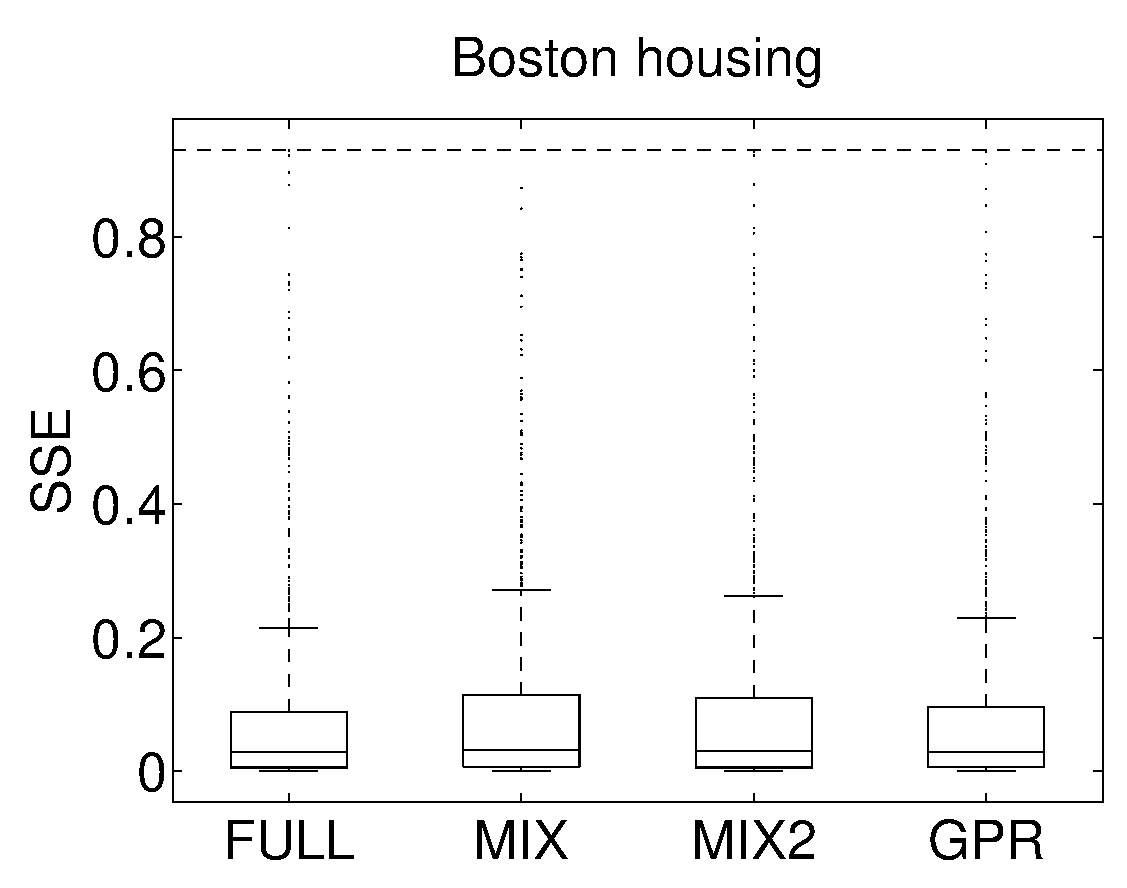
\includegraphics[scale=0.2]{figures/housing-smse.eps} &
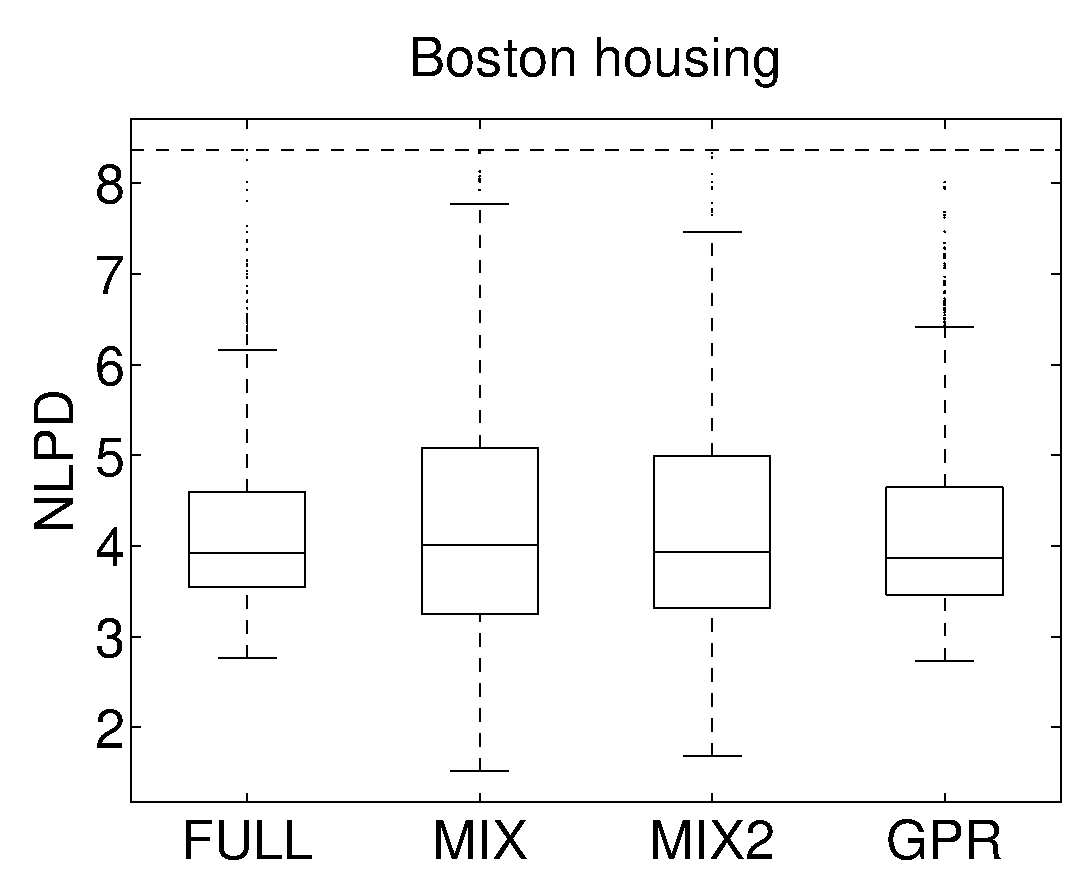
\includegraphics[scale=0.2]{figures/housing-nlpd.eps} \\
\end{tabular}
\caption{The distributions of SSE and NLPD of all methods on the regression task. Compared to the exact inference method GPR, the performance of AGP-FULL is identical while that of AGP-MIX and AGP-MIX2 are comparable.}
\label{fig:regression}
\end{figure*}

\subsection{Warped Gaussian processes (WGP)}
\begin{figure*}
\setlength{\tabcolsep}{0pt}
\begin{tabular}{cccc}
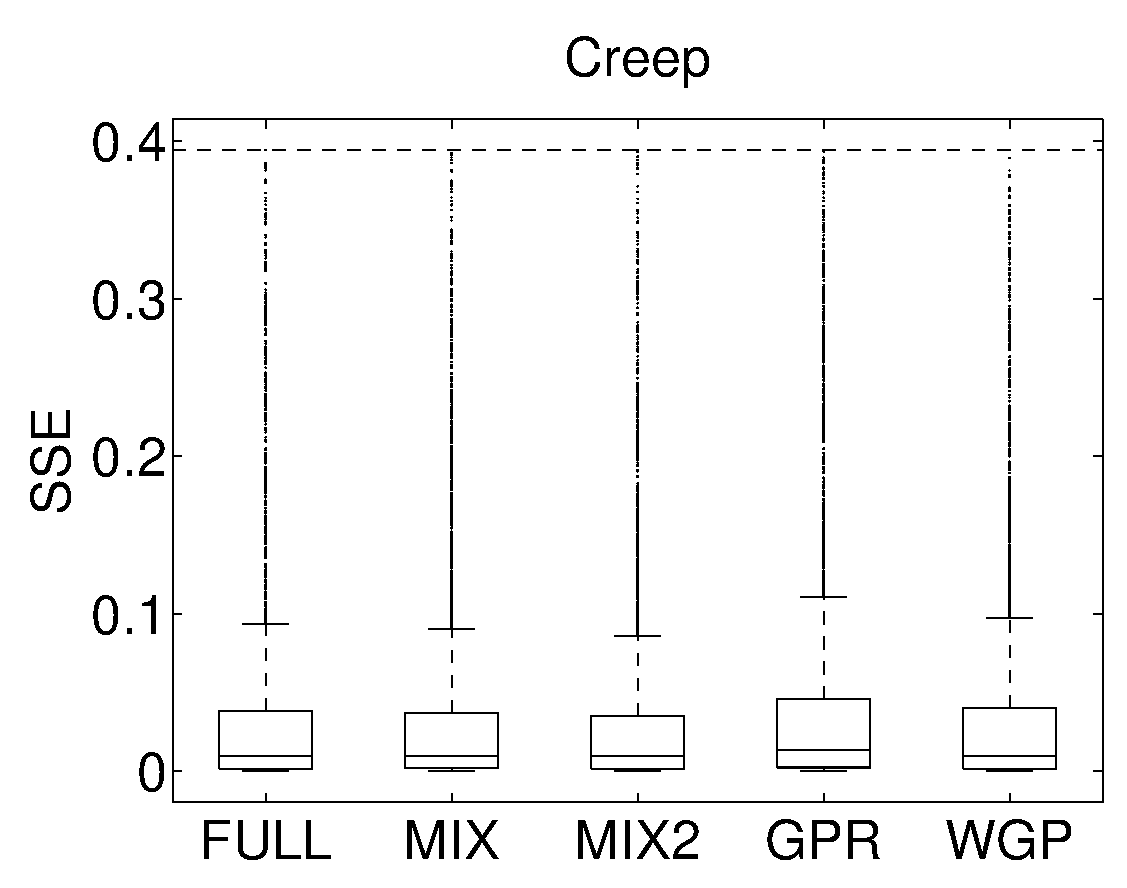
\includegraphics[width=0.25\linewidth]{figures/creep-smse.eps} &
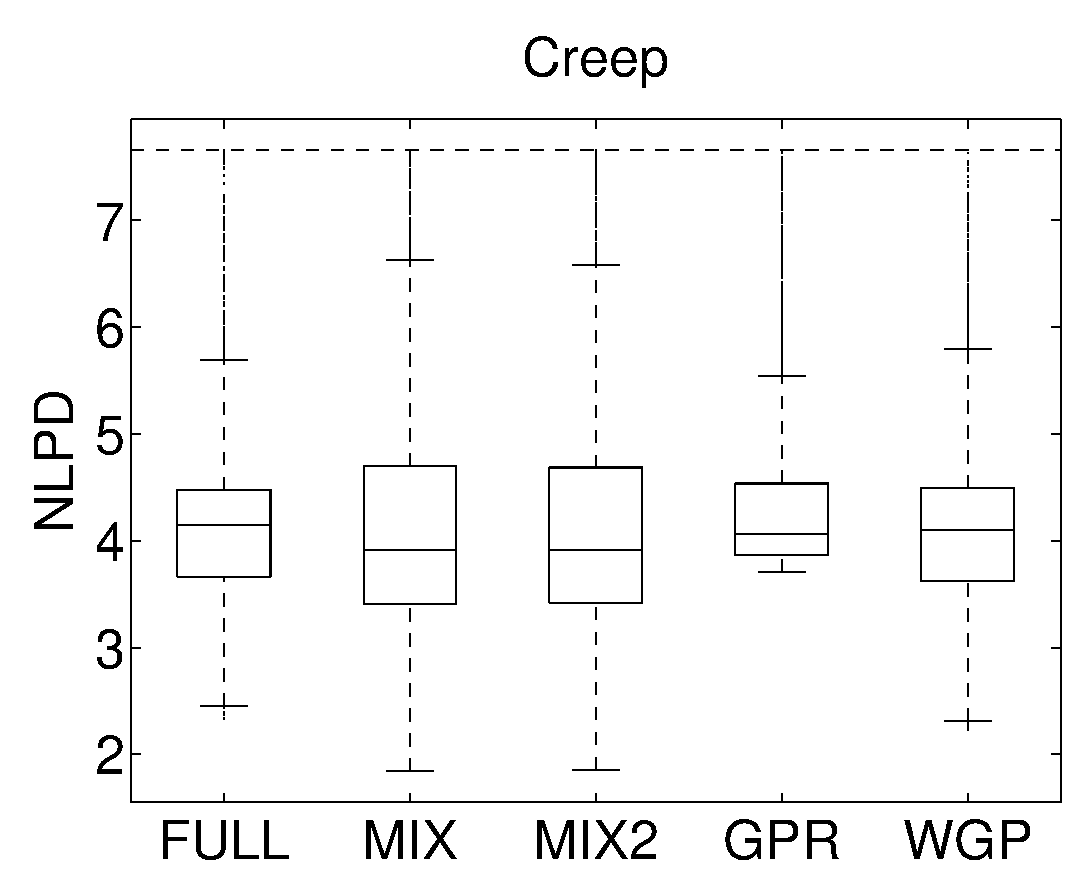
\includegraphics[width=0.24\linewidth]{figures/creep-nlpd.eps} &
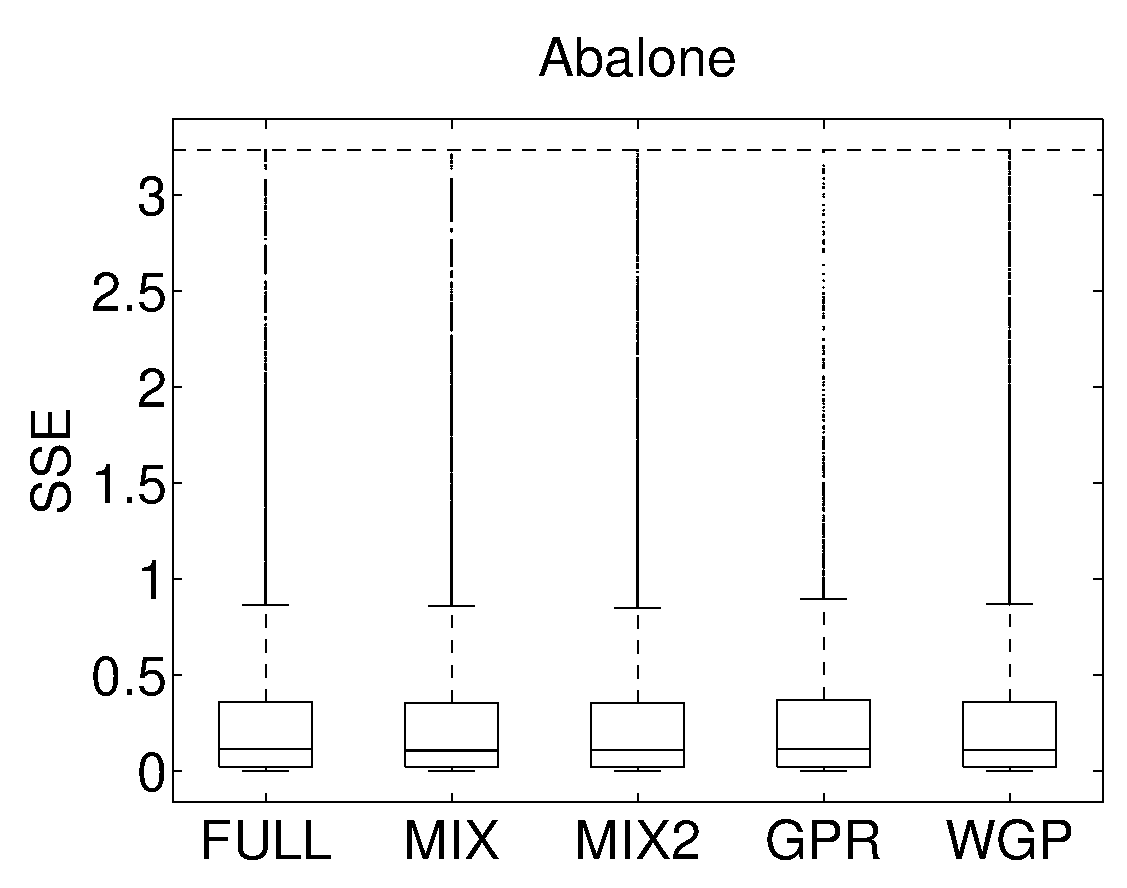
\includegraphics[width=0.25\linewidth]{figures/abalone-smse.eps} &
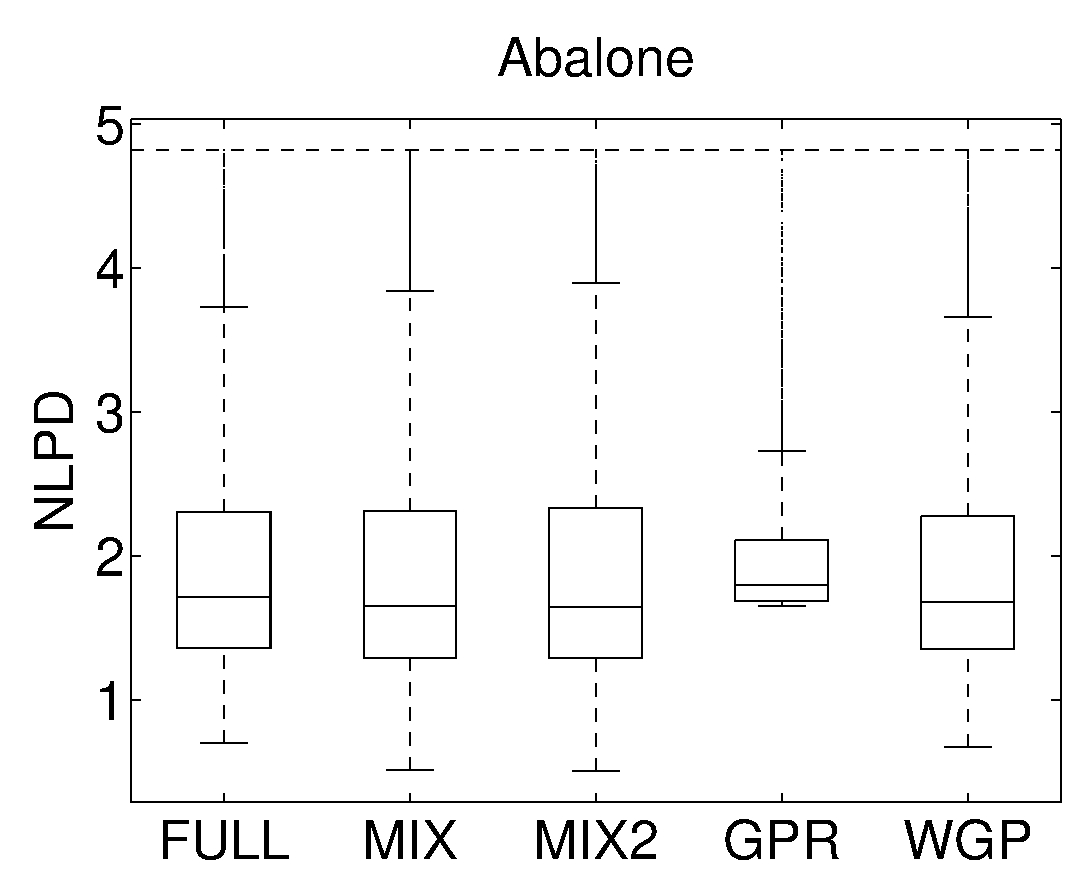
\includegraphics[width=0.24\linewidth]{figures/abalone-nlpd.eps} 
\end{tabular}
\caption{The distributions of SSE and NLPD of all methods on the regression task with warped GPs. 
The \agp \space methods ({\sc full}, {\sc mix} and {\sc mix2}) give comparable performance
to  exact inference with \wgp \space and slightly outperform \gpr \space which has  narrower ranges of predictive variances.}
\label{fig:warp}
\end{figure*}
%
The \wgp \space allows for non-Gaussian processes and non-Gaussian noises.
The likelihood for each target $y_n$ is attained by warping it through a nonlinear monotonic transformation $t(y)$ giving $p(y_n | f_n) = \nabla_{y_n} t(y_n) \Normal(t(y_n) | f_n, \sigma^2)$.
We used the same neural net style transformation %$t(y) = y + \sum_{i=1}^C a_i \tanh (b_i (y + c_i)), a_i, b_i \ge 0 \quad \forall i.$, where $a_i$, $b_i$, and $c_i$ parametrize $t(y)$
as in \cite{snelson2003warped}.
We fixed the warp parameters and used the same procedure for making analytical approximations to the predicted means and variances for all methods.

We compare with the exact implementation of \cite{snelson2003warped} %where the parameters are learned by optimizing the exact marginal likelihood.
and the standard GP regression (\gpr) on the Creep \cite{cole2000modelling} and Abalone \cite{uci2013} datasets.
%With Creep, the aim is to predict the creep rupture stress for steel given chemical composition and other inputs.
%With Abalone, the aim is to predict the age of abalone from various physical inputs.
The results in Figure \ref{fig:warp} show that the \agp \space methods give comparable performance to the exact  method \wgp \space and slightly outperform \gpr.  
The prediction by \gpr \space exhibits characteristically narrower ranges of predictive variances which can be attributed to its Gaussian noise assumption.

\subsection{Classification}
%For binary classification, the logistic likelihood $p(y_n = +1|f_n) = \frac{1}{1 + \exp(-f_n)}$ is chosen where $+1$ indicates the label of the positive class.
%The probability of the negative class with label $-1$ equals $1 - p(y_n = +1|f_n)$.
%For multiple classes, there are $C$ latent functions, $f_1$, $\hdots$, $f_C$, each associated with a different class.
%The latent function values at data point $n$ is collected into the vector $\f_{(n)} = [f_1(\x_n), \hdots, f_C(\x_n)]$ from which the softmax likelihood function can be constituted, 
%$p(\y_n | \f_{(n)}) = \frac{\sum_{i=1}^C \exp(y_{in} f_{in})}{\sum_{i=1}^C \exp(f_{in})}$.
%Here $f_{in} = f_i(\x_n)$ and $\y_n = \{y_{in}\}_{i=1}^C$ is a binary vector that has only an entry of 1 for the class label of the data point $n$.
%If we let that label be $c$, i.e., $y_{cn} = 1$ then the form given in Table \ref{tab:datasets} is recovered.
\begin{figure*}
\centering
\begin{tabular}{ccc}
\includegraphics[width=0.3\linewidth]{figures/classfication-errors.eps}  &
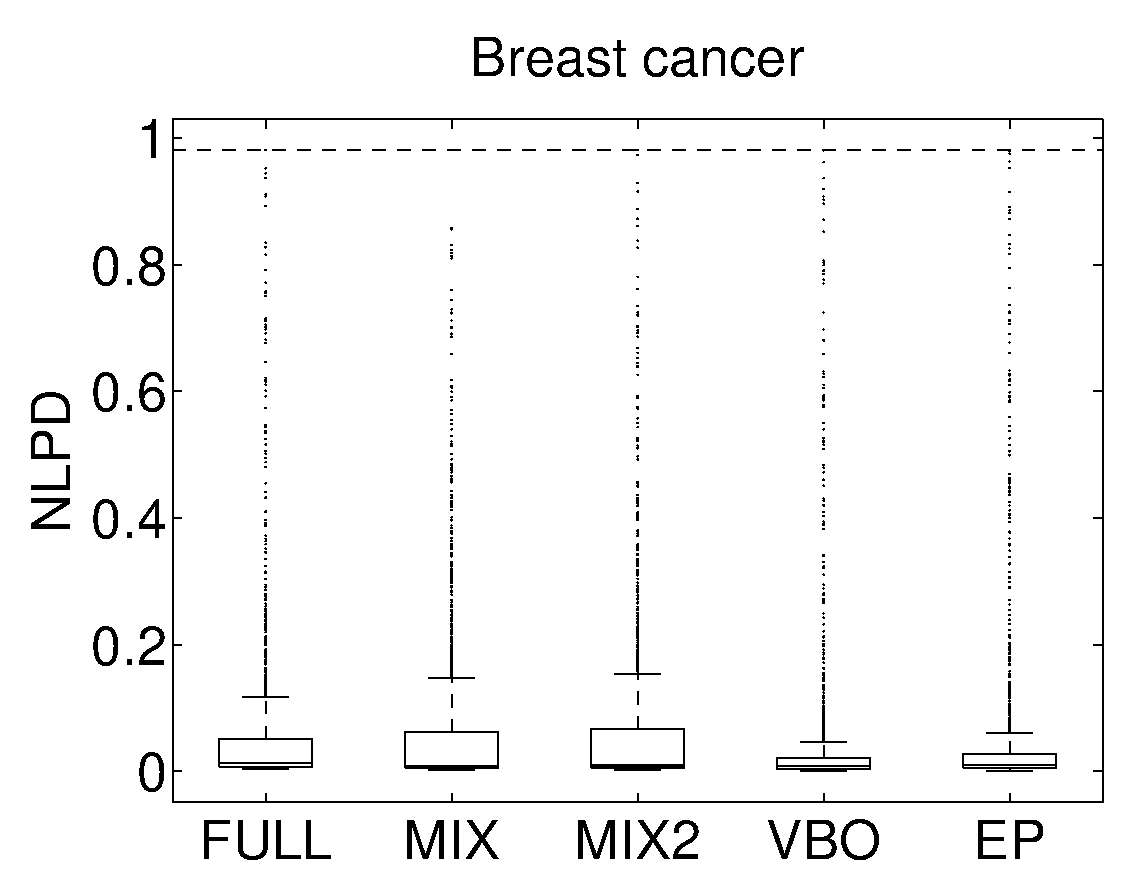
\includegraphics[width=0.3\linewidth]{figures/breast-nlpd.eps} &
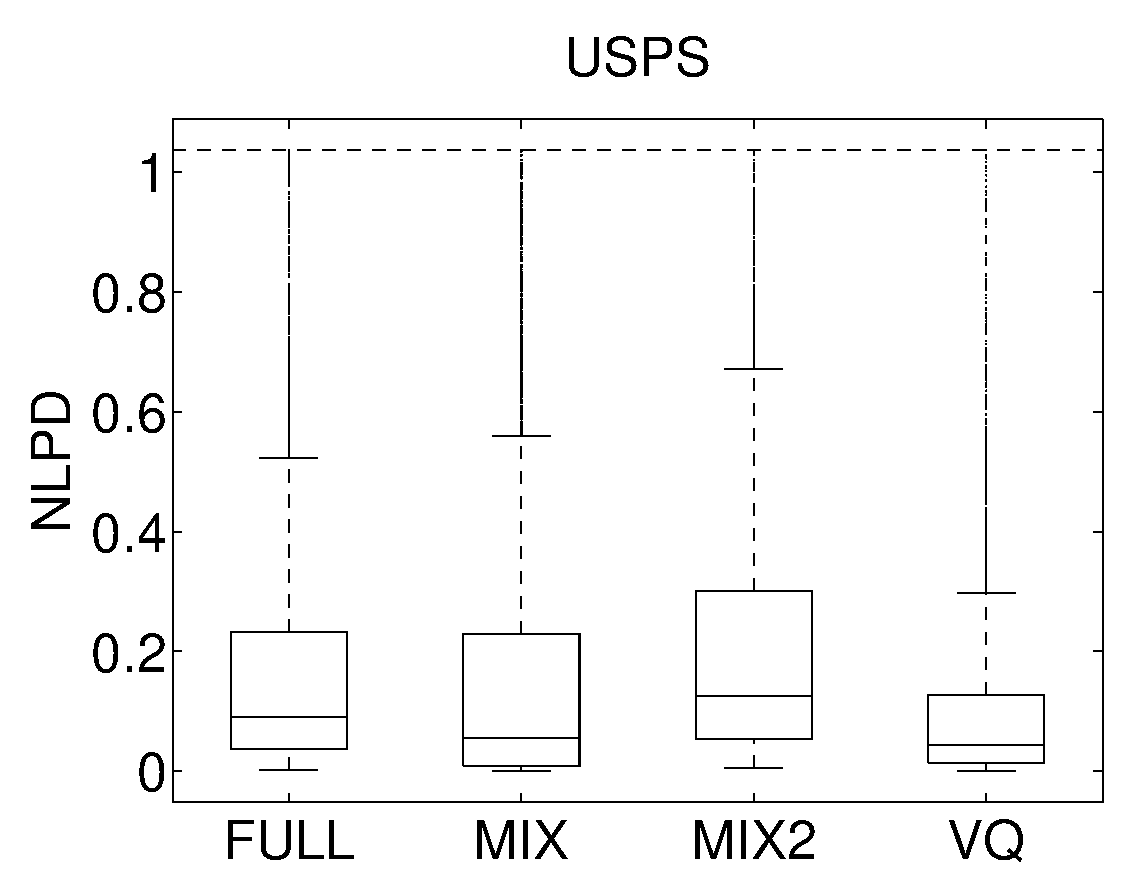
\includegraphics[width=0.3\linewidth]{figures/usps-nlpd.eps} 
\end{tabular}
\caption{\emph{Left plot}: classification error rates averaged over 5 runs (the error bars show two standard deviations). The \agp \space methods have classification errors comparable to the hard-coded implementations. \emph{Middle and right plots}: the distribution of NLPD of all methods on the binary and multi-class classification tasks, respectively. The hard-coded methods are slightly better than \agp.}
\label{fig:classification}
\end{figure*}

For binary classification, we use the logistic likelihood and experiment with the Wisconsin breast cancer 
 dataset \cite{uci2013}. %and the Ionosphere \cite{uci2013} datasets.
We compare with the variational bounds (\vbo) and the expectation propagation (\ep) methods.
%Note that \vbo \space is a local variational inference approach whose 
%ELBO is induced differently via a lower bound of the individual logistic likelihood. 
Details of \vbo \space and \ep \space can be found in  \cite{nickisch2008approximations}.
All  methods use the same analytical approximations when making prediction.

For multi-class classification, we use the softmax likelihood and experiment with a subset of the USPS dataset \cite{rasmussen-williams-book} containing the digits 4, 7, and 9.
We compare with a variational inference method  (\vq) which constructs the ELBO via a quadratic lower bound to the likelihood terms \cite{khan2012stick}.
Prediction is made by squashing the samples from the predictive distributions of the latent values at test points through the softmax likelihood for all methods.

The classification error rates and the NLPD are shown in Figure  \ref{fig:classification} for both tasks.
For binary classification, the \agp \space methods give comparable performance 
to the hard-coded implementations, \vbo \space and \ep. The latter is often considered the best approximation method for this task \cite{nickisch2008approximations}.
Similar results can be observed for the multi-class classification problem.
%The multi-modal posteriors \agpmixtwo \space do not seem to improve upon the uni-modal counterparts, suggesting that the true posterior may take the shape of a unimodal distribution.

We note that the running times of our methods are  comparable to that of the hard-coded methods.
For example, the average training times for \vbo, \ep, MIX, and FULL are 76s, 63s, 210s, and 480s respectively, on the Wisconsin dataset.

% previous figures with ionosphere
%\begin{figure*}
%\centering
%\begin{tabular}{c}
%\includegraphics[width=0.35\linewidth]{figures/classfication-errors.eps} 
%\end{tabular}
%\caption{Classification error rates on the binary and multi-class classification task. }
%\label{fig:classificationErrors}
%\end{figure*}

%\begin{figure*}
%\centering
%\begin{tabular}{ccc}
%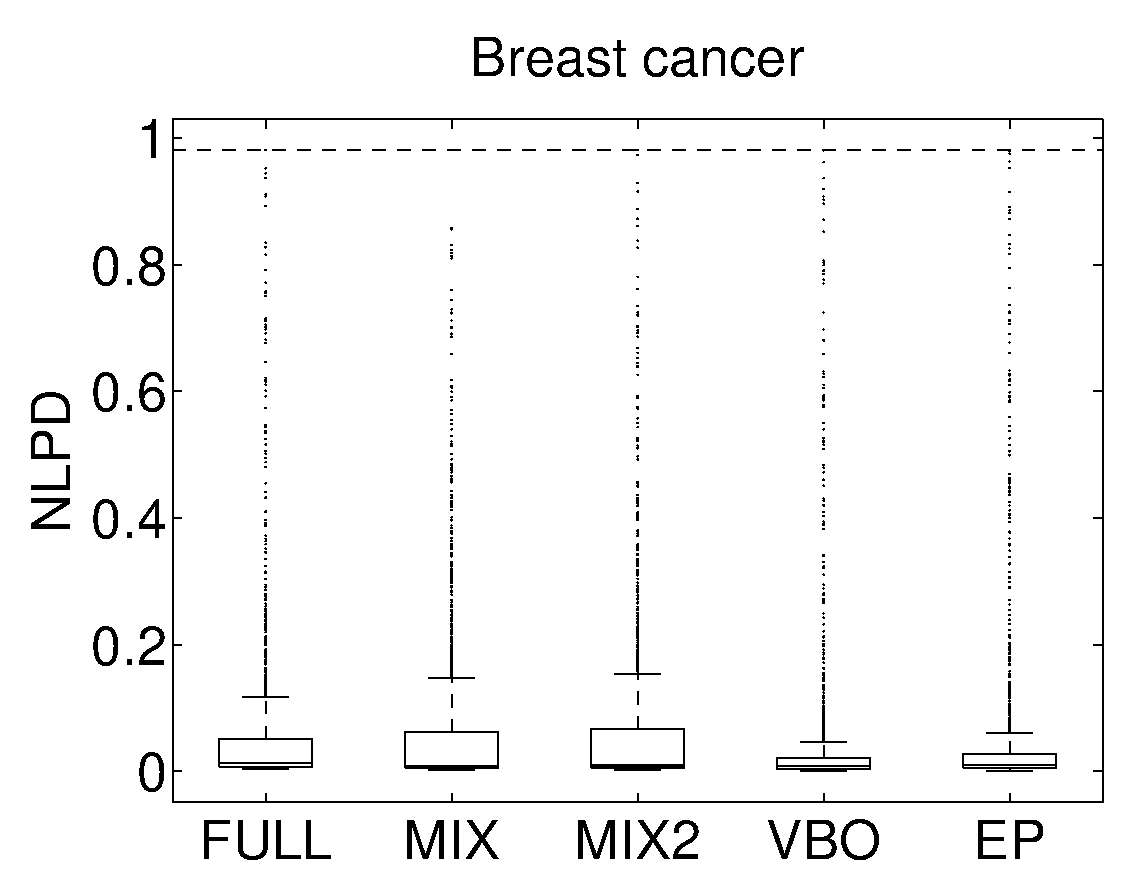
\includegraphics[width=0.25\linewidth]{figures/breast-nlpd.eps} &
%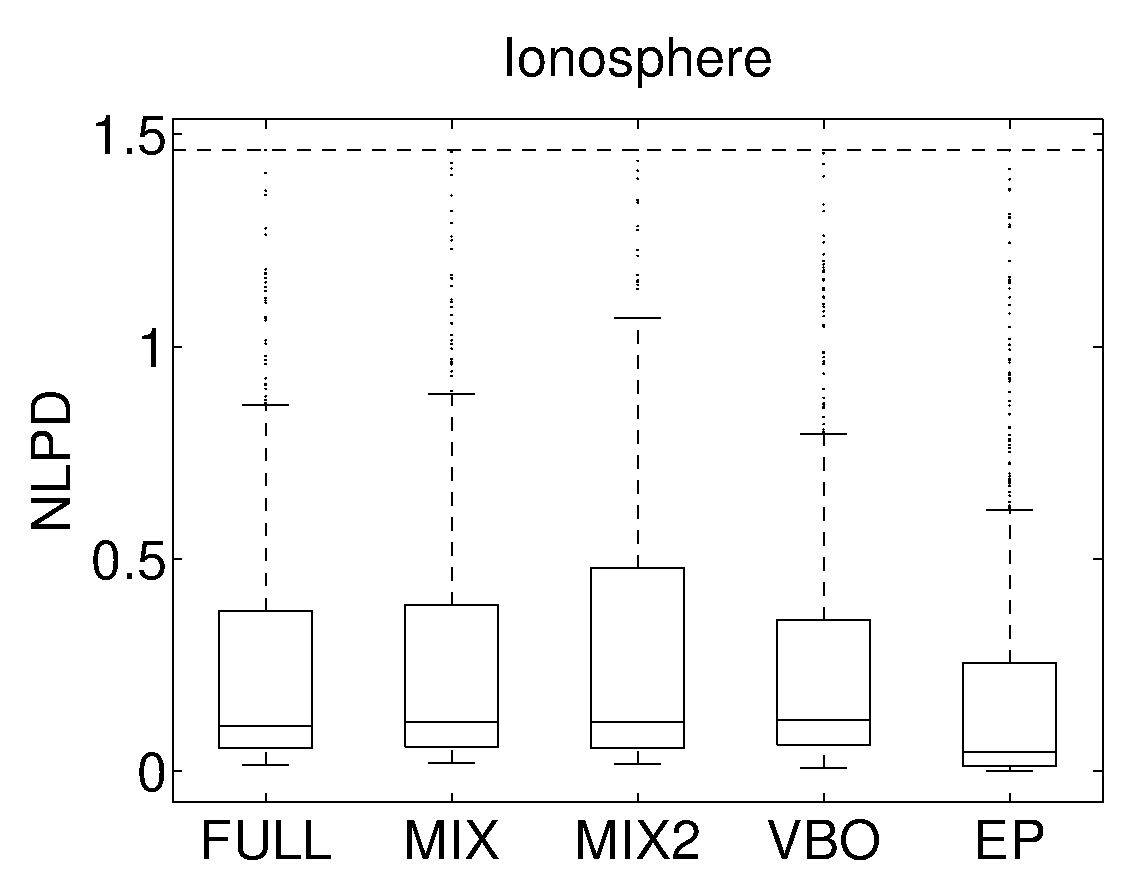
\includegraphics[width=0.25\linewidth]{figures/ionosphere-nlpd.eps} &
%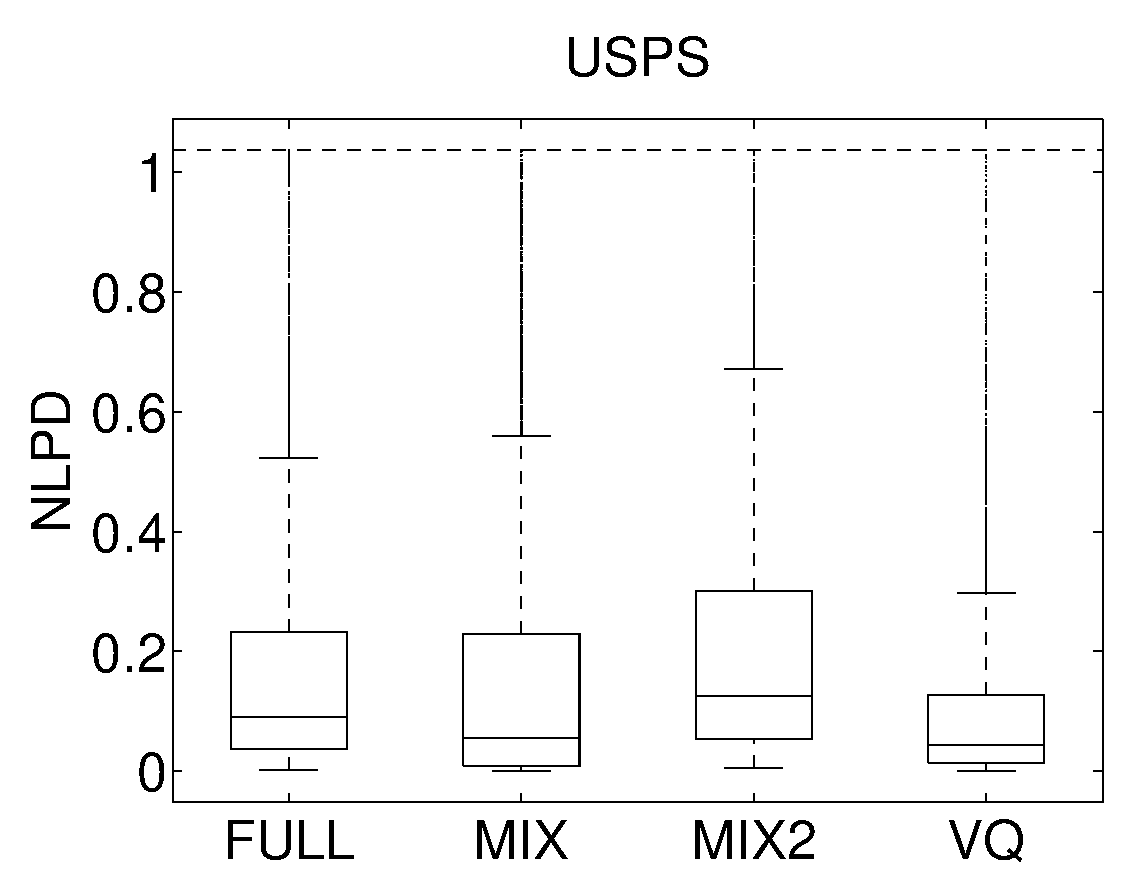
\includegraphics[width=0.25\linewidth]{figures/usps-nlpd.eps} 
%\end{tabular}
%\caption{Performance comparison on the binary and multi-class classification task. }
%\label{fig:classification}
%\end{figure*}

\subsection{Log Gaussian Cox process (LGCP) \label{sec:lgcp}}
The LGCP is an inhomogeneous Poisson process with the log-intensity function being a shifted draw from a Gaussian process.
Following \cite{murray2009elliptical}, we use the likelihood $p(y_n | f_n) = \frac{\lambda_n^{y_n} \exp(-\lambda_n)}{y_n!},$ where $\lambda_n = \exp(f_n + m)$ is the mean of a Poisson distribution and $m$ is the offset to the log mean. 
The data concerns  coal-mining disasters taken from a standard dataset for testing point processes \cite{jarrett1979note}.
The offset $m$ and the covariance hyperparameters are set to the same values as in \cite{murray2009elliptical}.
%The 191 events were placed into 811 bins of 50 days each. 
%The offset $m$ is set to $m = log(191/811)$ and the covariance hyperparameters fixed to $\sigma_f^2 = 1$ and $l = 13516$.
%The covariance hyperparameters are fixed to $\sigma_f^2 = 1$ and $l = 13516$.

We compare \agp \space with the  Hybrid Monte Carlo (\hmc, \cite{duane1987hybrid}) and 
elliptical slice sampling  (\ess, \cite{murray2009elliptical}) methods, where the latter is designed specifically for GP models.
We collected every $100$th sample for a total of $10$k samples after a burn-in period of $5$k samples; the  Gelman-Rubin potential scale reduction factors \citep{gelman1992inference} are used to check for convergence. 
%In Figure \ref{fig:loggcp}, the left plot shows the true event counts per 50 days during the given time period.
%The middle plot shows the posteriors by all methods.
The middle plot of Figure \ref{fig:loggcp} shows the posteriors learned by all methods.
 We see that the posterior by \agpfull \space is 
 similar to that 
by \hmc \ and \ess.
\agpmix \space obtains the same posterior mean but it underestimates the variance. 
%Note that the predictive mean of all methods will be the same as it does not depend on the variance of the posterior.
The right plot shows the speed-up factors of all methods against the slowest method \hmc. % -- the slowest method. which took $196$ minutes, in $\log_{10}$ scale.
The \agp \space methods run more than two orders of magnitude faster than \hmc, thus confirming the computational advantages of our method to the sampling approaches.
Training time was measured on a desktop with Intel(R) i7-2600 3.40GHz CPU with 8GB of RAM using Matlab R2012a.
\begin{figure*}
\centering
\begin{tabular}{ccc}
\includegraphics[width=0.3\linewidth]{figures/loggcp-intensity.eps} &
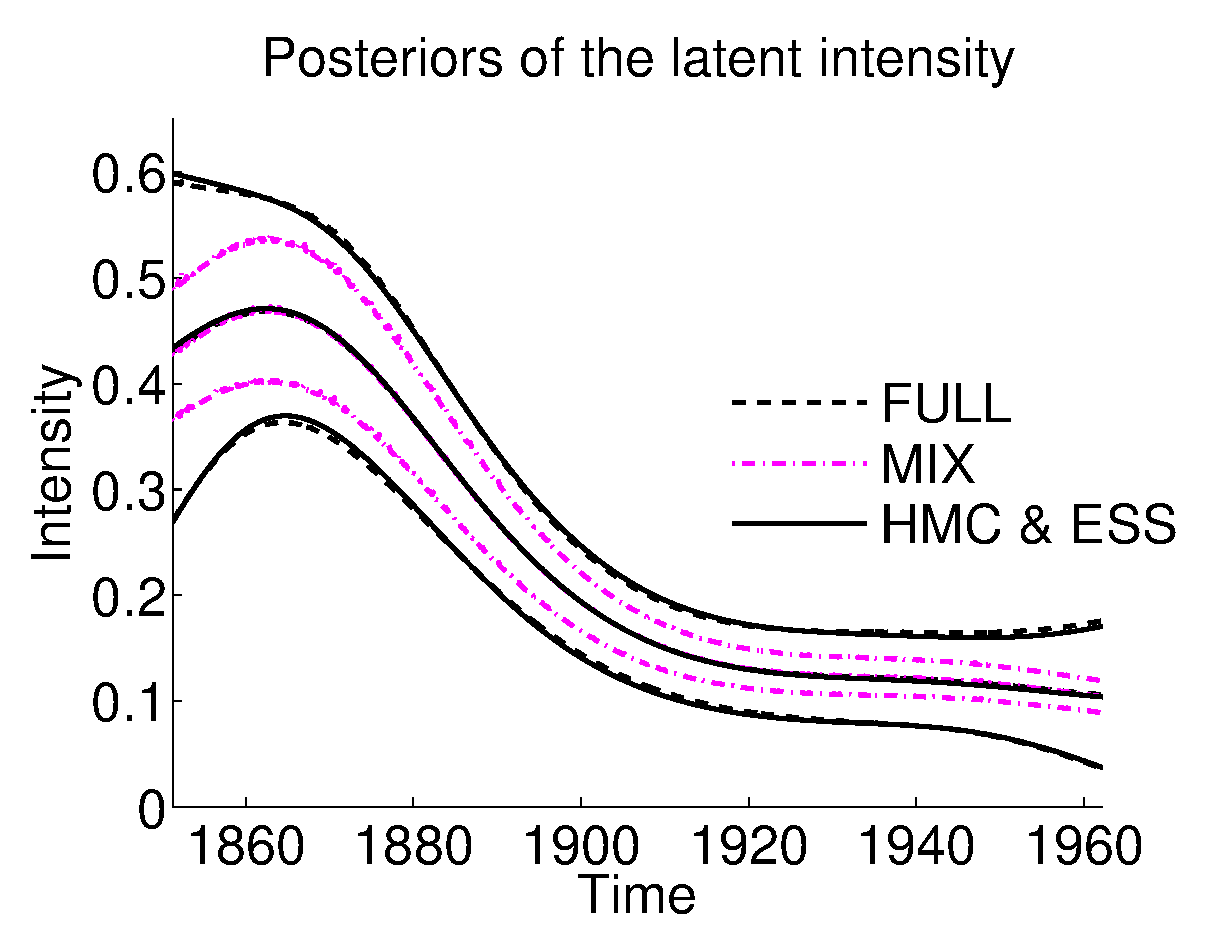
\includegraphics[width=0.3\linewidth]{figures/loggcp.eps} &
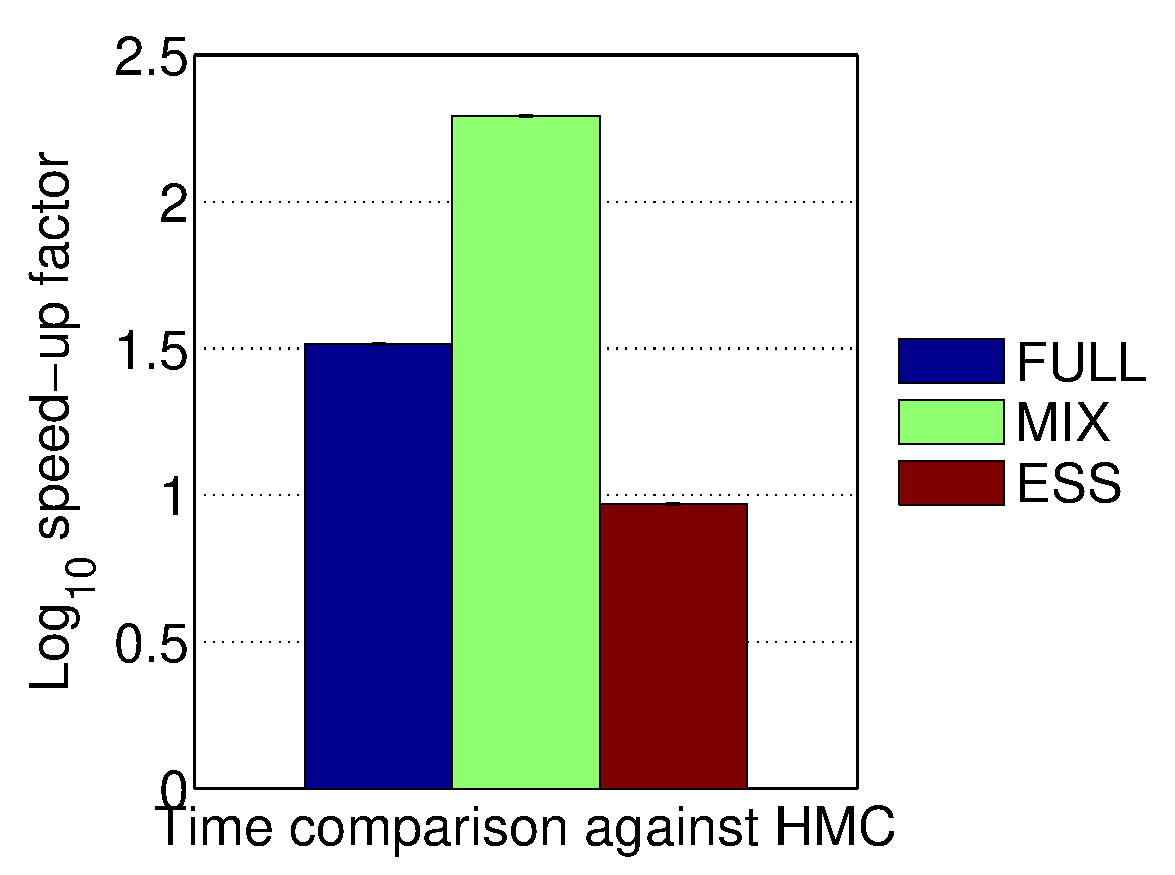
\includegraphics[width=0.3\linewidth]{figures/loggcp-time.eps}
\end{tabular}
\caption{\emph{Left plot}: the true event counts during the given time period. \emph{Middle plot}: the posteriors (estimated intensities) inferred by all methods. For each method, the middle line is the posterior mean and the two remaining lines enclose 90\% interval. \agpfull \space infers the same posterior as \hmc \space and \ess \space while \agpmix \space obtains the same mean but underestimates the variance. \emph{Right plot}: speed-up factors against the HMC method. The \agp \space methods run more than 2 orders of magnitude faster than the sampling methods. %The posterior distributions are virtually identical for the two sampling methods and the variational inference with full posterior. The diagonal posterior underestimates the variance, but the mean is the same as all other methods.
}
\label{fig:loggcp}
\end{figure*}

%\subsection{Toy Classification}
%Here I used a toy classifcation dataset (generated by the \textit{demoClassification} script in the GPML package). 
%The samples are generated from two Gaussian with different means and covariance.
%\paragraph{Prediction}
%The data and predictive probabilities of the test data points being in the positive class by the exact variational inference (\textbf{exactVB}), black box inference (\textbf{blackbox}), inference with a full Gaussian posterior (\textbf{fullGaussian}) and mixture of Gaussians posterior (\textbf{mixture}) are shown in Figure \ref{fig:toy}.
%It can be seen that black box inference fails to work (in fact the variance increases as the algorithm progresses).
%
%\begin{figure*}
%\centering
%\begin{tabular}{cc}
%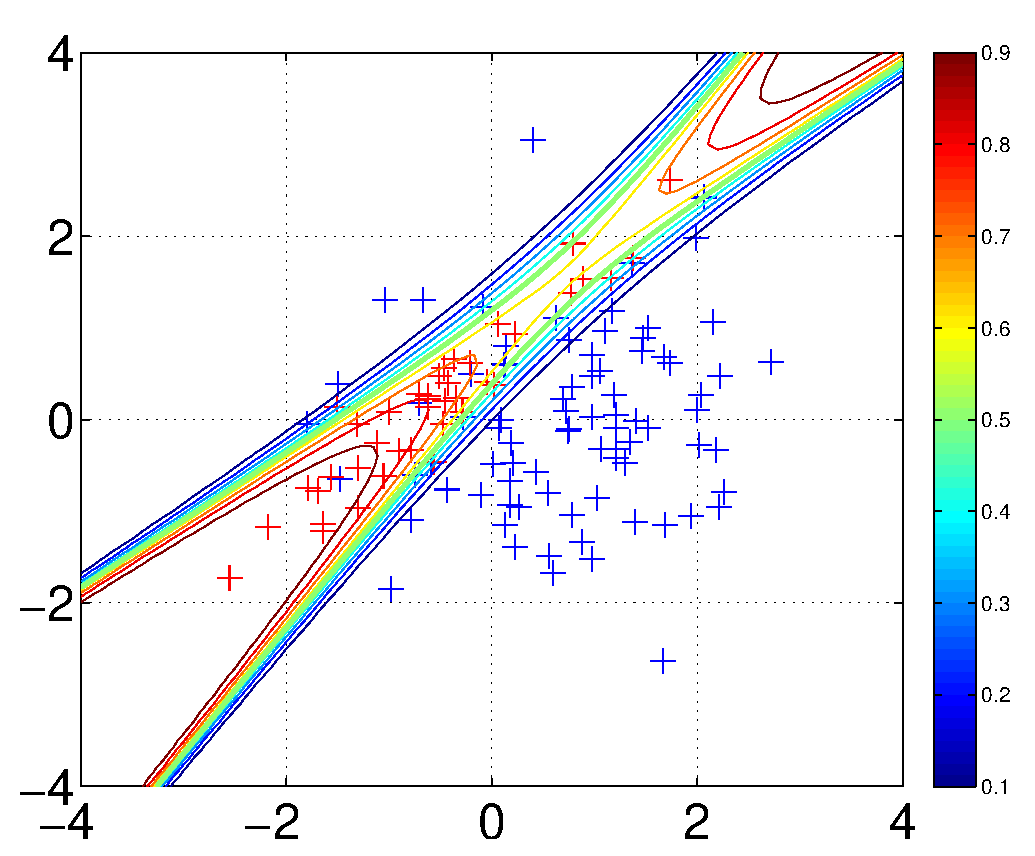
\includegraphics[scale=0.4]{figures/f6.eps} &
%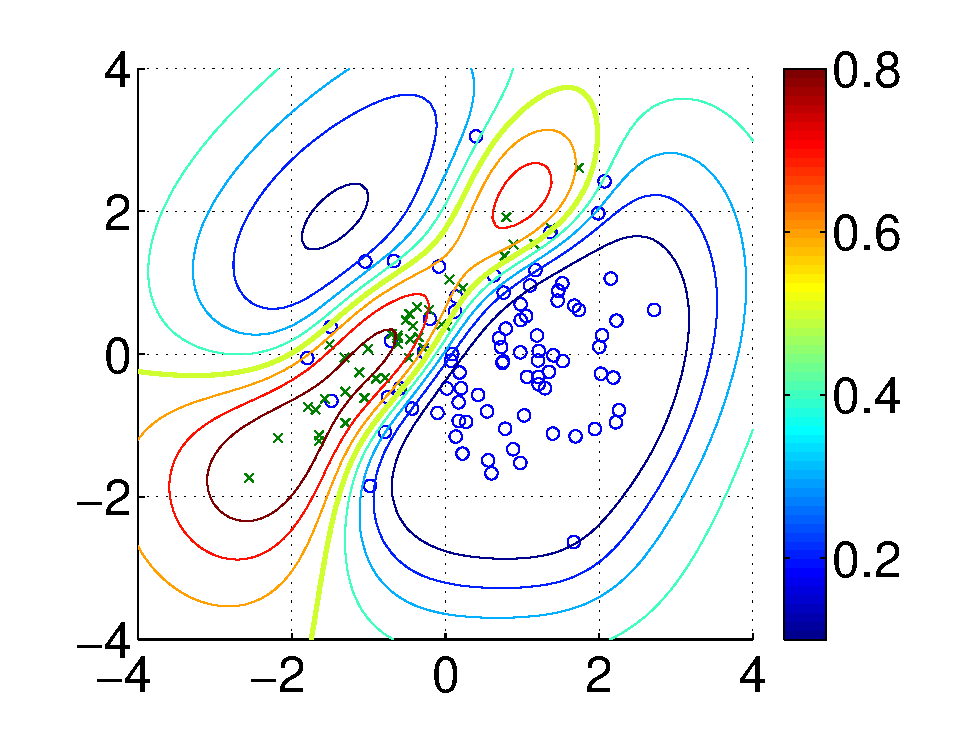
\includegraphics[scale=0.5]{figures/exactVB.eps} \\
%data & exactVB  \\
%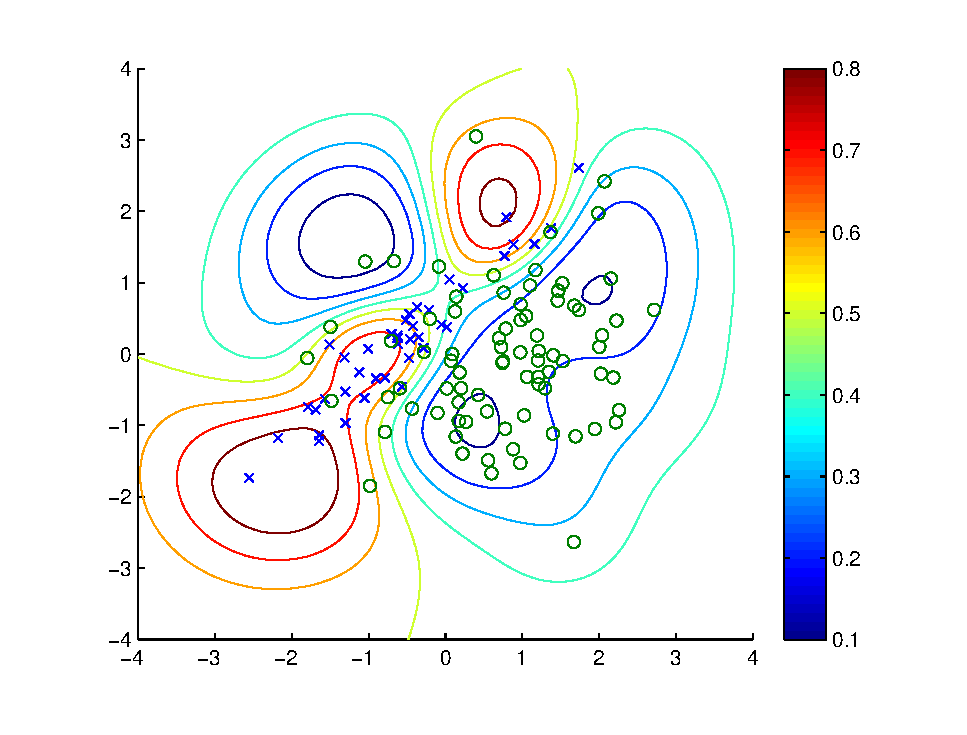
\includegraphics[scale=0.5]{figures/fullgaus-iter100-largelrate.eps} &
%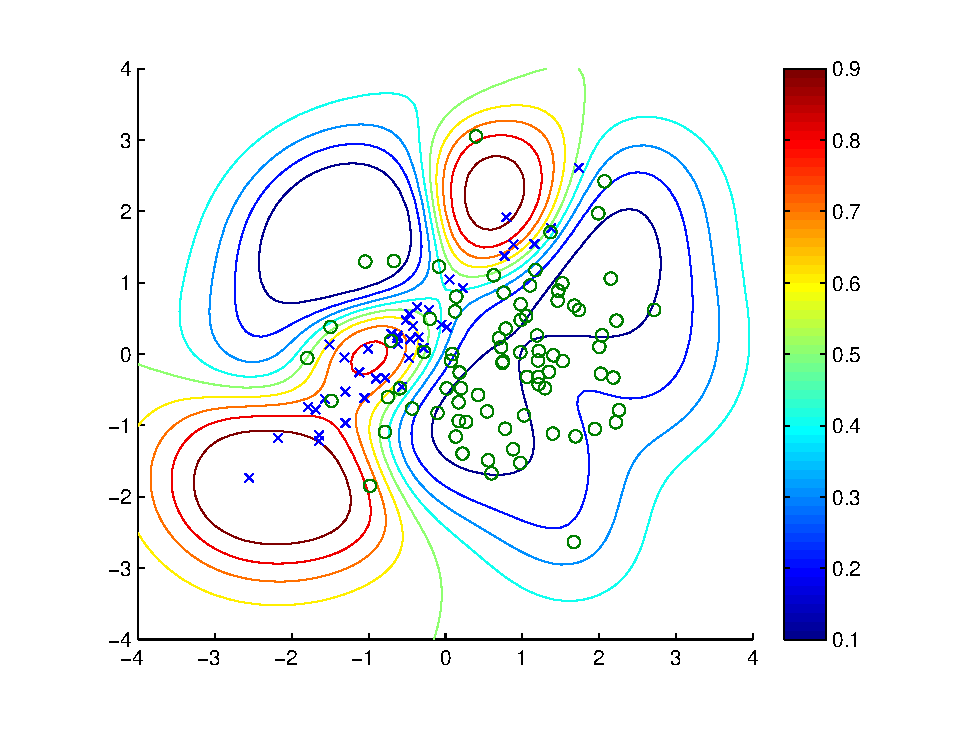
\includegraphics[scale=0.5]{figures/mixture-iter100-largelrate.eps} \\
%fullGaussian & mixture \\
%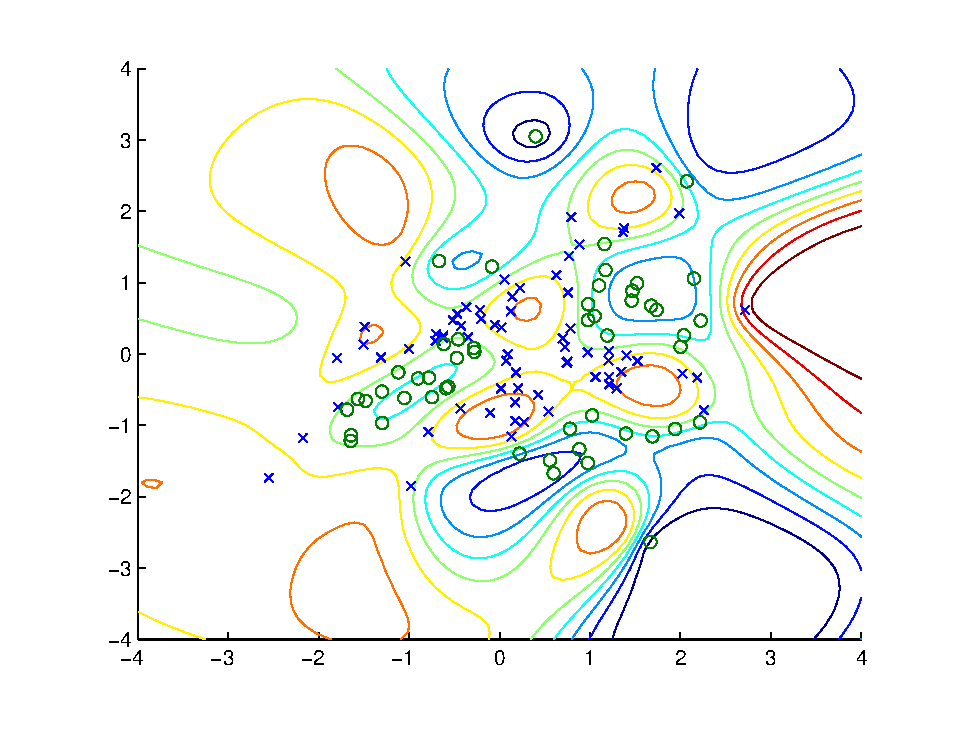
\includegraphics[scale=0.5]{figures/blackbox.eps} & \\
%blackbox
%\end{tabular}
%\caption{Data and the contour of predictive probability of data points being classified as positive. The dots are training data points. (The marker for the 2 classes of exactVB should be switched, but the contour means the same thing!)}
%\label{fig:toy}
%\end{figure*}
%
%\paragraph{Variances of the estimators}
%The average variances of the gradient estimators are $3$ and $1e4$ for the mixture (with one component) and  full Gaussian, respectively. The variance for black box inference is $1e8$ with 10,000 samples and $1e10$ with 2000 samples.
%It is clear that merely increasing the number of samples is not effective in reducing the variance.
%
%\paragraph{Training time}
%Training time for the mixture with one component (100 iterations) takes around 1 minute.
%Training time for full Gaussian (also with 100 iterations) is around 10 minutes.
%Training time for black box inference (also with 100 iterations) is around 20 minutes. The additional cost is due to sampling to estimate the gradient of the hyperparameters and also due to computing the entropy and cross-entropy which are analytic in our proposal.

